%========================abstract=========================
\section*{Executive Summary}
%\addcontentsline{toc}{section}{Abstract}
\noindent Agricultural intensification, mechanization, and automation have all led to major increases in agricultural productivity throughout time \cite{nof2009springer}. Robots are intelligent machines that may be trained to carry out particular jobs, make choices, and take immediate action. They are needed in a variety of industries where less labor is often needed, and they function best in stable environments where consistent accuracy and high productivity are required \cite{nof1999handbook}.\\
~\\
\noindent LEF BOTS GmbH is a robot specialising company, the name of the firm is created from the initials of the stakeholders: \textbf{L}aura; \textbf{E}ncarnacion; \textbf{F}erlando \textbf{(LEF)}. In this text, the firm presents the development of its major product; the fruit harvesting robot. The robot is given an intuitive name \textbf{Fruta Oes}, which is a combination of two languages Spanish and Afrikaans. Fruta means fruits in Spanish and Oes means to harvest in Afrikaans, thus, the name of the robot \textbf{Fruta Oes} means fruits harvester. One might be asking themselves why Spanish and Afrikaans, well the answer is simple, the stakeholders of the firm are from Spain (Laura and Encarnacion) and South Africa (Ferlando). \Vref{fig:2oppositeviews} Presents \textbf{Fruta Oes}.
\begin{figure}[h]
	\centering
	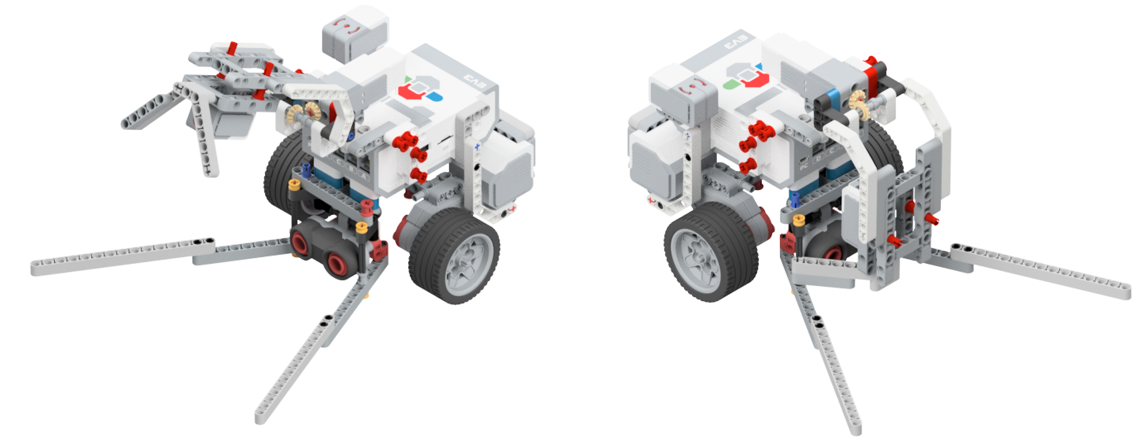
\includegraphics[width=\linewidth]{Graphics/2oppositeViews}
	\caption{Fruta Oes}
	\label{fig:2oppositeviews}
\end{figure}

\noindent The robot mechanical structure is the most important part of this project therefore, this document will discuss in detail all the sub-components of the mechanical design in \vref{sec:mechanicalDesign}. Following by the software design where a full discussion on all the algorithms used, activity diagrams and testing will be provided in \vref{sec:softwareDesign}. Following will be the management of the software development, \vref{sec:softwareEngineering} highlights the Agile Software engineering (SCRUM) procedure followed in this project. The SCRUM section will briefly discuss the project setup in \vref{sec:projectSetup}, then \cref{sec:sprint1}, \cref{sec:sprint2},\cref{sec:sprint3} present the role and progress achieved in sprint 1, sprint 2 and sprint 3 respectively. Finally, recommendations will be detailed in \vref{sec:RecommendationsAndConclusion} then in the same section this document will go into a concluding discussion.









